\documentclass{article}

\usepackage[export]{adjustbox}
\usepackage{algorithmic}
\usepackage{amsmath}
\usepackage{amssymb}
\usepackage{amsthm}
\usepackage{dsfont}
\usepackage{commath}
\usepackage{graphicx}
\usepackage{hyperref}
\usepackage[utf8]{inputenc}
\usepackage{amsfonts}
\usepackage{bm}

\newcommand{\bba}{{\mathbb A}}
\newcommand{\bbb}{{\mathbb B}}
\newcommand{\bbc}{{\mathbb C}}
\newcommand{\bbd}{{\mathbb D}}
\newcommand{\bbe}{{\mathbb E}}
\newcommand{\bbf}{{\mathbb F}}
\newcommand{\bbg}{{\mathbb G}}
\newcommand{\bbh}{{\mathbb H}}
\newcommand{\bbi}{{\mathbb I}}
\newcommand{\bbj}{{\mathbb J}}
\newcommand{\bbk}{{\mathbb K}}
\newcommand{\bbl}{{\mathbb L}}
\newcommand{\bbm}{{\mathbb M}}
\newcommand{\bbn}{{\mathbb N}}
\newcommand{\bbo}{{\mathbb O}}
\newcommand{\bbp}{{\mathbb P}}
\newcommand{\bbq}{{\mathbb Q}}
\newcommand{\bbr}{{\mathbb R}}
\newcommand{\bbs}{{\mathbb S}}
\newcommand{\bbt}{{\mathbb T}}
\newcommand{\bbu}{{\mathbb U}}
\newcommand{\bbv}{{\mathbb V}}
\newcommand{\bbw}{{\mathbb W}}
\newcommand{\bbx}{{\mathbb X}}
\newcommand{\bby}{{\mathbb Y}}
\newcommand{\bbz}{{\mathbb Z}}

\newcommand{\bma}{{\bm a}}
\newcommand{\bmb}{{\bm b}}
\newcommand{\bmc}{{\bm c}}
\newcommand{\bmd}{{\bm d}}
\newcommand{\bme}{{\bm e}}
\newcommand{\bmf}{{\bm f}}
\newcommand{\bmg}{{\bm g}}
\newcommand{\bmh}{{\bm h}}
\newcommand{\bmi}{{\bm i}}
\newcommand{\bmj}{{\bm j}}
\newcommand{\bmk}{{\bm k}}
\newcommand{\bml}{{\bm l}}
\newcommand{\bmm}{{\bm m}}
\newcommand{\bmn}{{\bm n}}
\newcommand{\bmo}{{\bm o}}
\newcommand{\bmp}{{\bm p}}
\newcommand{\bmq}{{\bm q}}
\newcommand{\bmr}{{\bm r}}
\newcommand{\bms}{{\bm s}}
\newcommand{\bmt}{{\bm t}}
\newcommand{\bmu}{{\bm u}}
\newcommand{\bmv}{{\bm v}}
\newcommand{\bmw}{{\bm w}}
\newcommand{\bmx}{{\bm x}}
\newcommand{\bmy}{{\bm y}}
\newcommand{\bmz}{{\bm z}}

\newcommand{\bmxi}{{\bm \xi}}

\newcommand{\bmA}{{\bm A}}
\newcommand{\bmB}{{\bm b}}
\newcommand{\bmC}{{\bm c}}
\newcommand{\bmD}{{\bm d}}
\newcommand{\bmE}{{\bm e}}
\newcommand{\bmF}{{\bm f}}
\newcommand{\bmG}{{\bm g}}
\newcommand{\bmH}{{\bm h}}
\newcommand{\bmI}{{\bm i}}
\newcommand{\bmJ}{{\bm j}}
\newcommand{\bmK}{{\bm k}}
\newcommand{\bmL}{{\bm l}}
\newcommand{\bmM}{{\bm m}}
\newcommand{\bmN}{{\bm n}}
\newcommand{\bmO}{{\bm o}}
\newcommand{\bmP}{{\bm p}}
\newcommand{\bmQ}{{\bm q}}
\newcommand{\bmR}{{\bm r}}
\newcommand{\bmS}{{\bm s}}
\newcommand{\bmT}{{\bm t}}
\newcommand{\bmU}{{\bm u}}
\newcommand{\bmV}{{\bm v}}
\newcommand{\bmW}{{\bm w}}
\newcommand{\bmX}{{\bm x}}
\newcommand{\bmY}{{\bm y}}
\newcommand{\bmZ}{{\bm z}}

\newcommand{\cala}{{\mathcal A}}
\newcommand{\calb}{{\mathcal B}}
\newcommand{\calc}{{\mathcal C}}
\newcommand{\cald}{{\mathcal D}}
\newcommand{\cale}{{\mathcal E}}
\newcommand{\calf}{{\mathcal F}}
\newcommand{\calg}{{\mathcal G}}
\newcommand{\calh}{{\mathcal H}}
\newcommand{\cali}{{\mathcal I}}
\newcommand{\calj}{{\mathcal J}}
\newcommand{\calk}{{\mathcal K}}
\newcommand{\call}{{\mathcal L}}
\newcommand{\calm}{{\mathcal M}}
\newcommand{\caln}{{\mathcal N}}
\newcommand{\calo}{{\mathcal O}}
\newcommand{\calp}{{\mathcal P}}
\newcommand{\calq}{{\mathcal Q}}
\newcommand{\calr}{{\mathcal R}}
\newcommand{\cals}{{\mathcal S}}
\newcommand{\calt}{{\mathcal T}}
\newcommand{\calu}{{\mathcal U}}
\newcommand{\calv}{{\mathcal V}}
\newcommand{\calw}{{\mathcal W}}
\newcommand{\calx}{{\mathcal X}}
\newcommand{\caly}{{\mathcal Y}}
\newcommand{\calz}{{\mathcal Z}}


\title{Neural Networks}
\author{Yu Gai}

\DeclareMathOperator*{\argmin}{arg\,min}
\DeclareMathOperator{\degree}{deg}
\DeclareMathOperator{\diag}{diag}
\DeclareMathOperator{\range}{range}

\newcommand{\ind}{{\mathds 1}}
\newcommand{\pp}[2]{{\frac{\partial {#1}}{\partial {#2}}}}

\newtheorem{definition}{Definition}
\newtheorem{corollary}{Corollary}
\newtheorem{lemma}{Lemma}
\newtheorem{theorem}{Theorem}

\begin{document}

\maketitle

\tableofcontents

\newpage

\section{Basics}

\subsection{The probably approximately correct (PAC) learning framework}

For ease of exposition, we restrict ourselves to the probably approximately correct (PAC) learning framework, where there is
\begin{itemize}
\item an input space $\calx \subset \bbr^d$
\item an output space $\caly$, e.g. $\{\pm 1\}$ (binary classification), and $\bbr$ (regression)
\item a probability measure $\bbp$ over the input space $\calx$
\item an (unknown) mapping that assigns desired output to input $y: \calx \mapsto \caly$
\item an i.i.d. sample $\{(\bmx_i, y_i)\}_{i = 1}^n$, where $\bmx_i \in \calx$ is sampled from $\bbp$ and $y_i = y(\bmx_i)$
\end{itemize}

\subsection{Empirical risk minimization (ERM)}

A hypothesis $h$ is a mapping $\calx \mapsto \caly$ (possibly different from $y$).
The true risk of a hypothesis $h$ is defined as
\[
R(h)
\triangleq \bbp \{h(\bmx) \ne y(\bmx)\}
= \bbe_\bmx \ell (h(\bmx), y(\bmx))
\]
Empirical risk minimization (ERM) refers to the approach to hypothesis search that returns a/the minimizer of an empirical risk in a hypothesis space.
Mathematically, given a hypothesis $h: \calx \mapsto \caly$, a loss function $\ell: \caly \times \caly$, and an i.i.d. sample $\{(\bmx_i, y_i)\}_{i = 1}^n \subset \calx \times \caly \mapsto \bbr$, the empirical risk is defined as
\[
\hat{R} (h) \triangleq \frac1n \sum_{i = 1}^n \ell (h(\bmx_i), y_i)
\]
In the case that $\caly = \{\pm 1\}$ and $\ell (y, y') = \ind_{y \ne y'}$,
\[
\hat{R} (h) = \frac1n \sum_{i = 1}^n \ind_{h(\bmx_i) \ne y_i}
\]
In the case that $\caly = \bbr$ and $\ell (y, y') = (y - y')^2$,
\[
\hat{R} (h) = \frac1n \sum_{i = 1}^n (h(\bmx_i) - y_i)^2
\]
\[
\argmin_{h \in \calh} \hat{R} (h)
\]

\subsection{Rosenblatt's Perceptron}

Frank Rosenblatt proposed his Perceptron in 1957 \cite{rosenblatt1958perceptron}.
Consider the case $\caly = \bbr$.
The hypothesis space of perceptrons is
\[
\calh \triangleq \{h_{\bmw, b} : \bmw \in \bbr^d, b \in \bbr\}
\]
where
\[
h_{\bmw, b} (\bmx)
\triangleq \bmw^T \bmx + b
= \sum_{i = 1}^d \bmw_i \bmx_i + b
\]
is a perceptron.
The components of an input $\bmx \subset \calx$ are conventionally referred to as features, and Rosenblatt's Perceptron returns a linear combination of input features plus a bias.
From now on we will refer to a linear combination plus a constant as a ``linear" combination for brevity.
The parameters $\bmw$ and $b$ may be chosen as
\begin{align*}
\argmin_{\bmw, b} \ell (\bmw, b)
& = \argmin_{\bmw, b} \frac1n \sum_{i = 1}^n (h_{\bmw, b} (\bmx_i) - y_i)^2 \\
& = \argmin_{\bmw, b} \frac1n \sum_{i = 1}^n (\bmw^T \bmx_i + b - y_i)^2
\end{align*}
which is an application of ERM with the quadratic loss function.

\subsubsection{Interpretation of Rosenblatt's Perceptron as neuron}

\begin{figure}
\centering
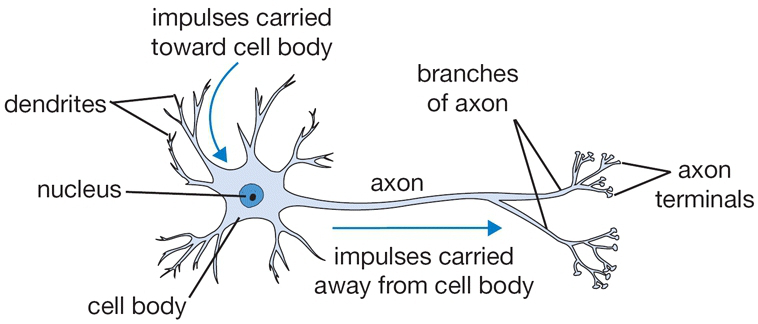
\includegraphics[scale=0.2, valign=t]{neuron}
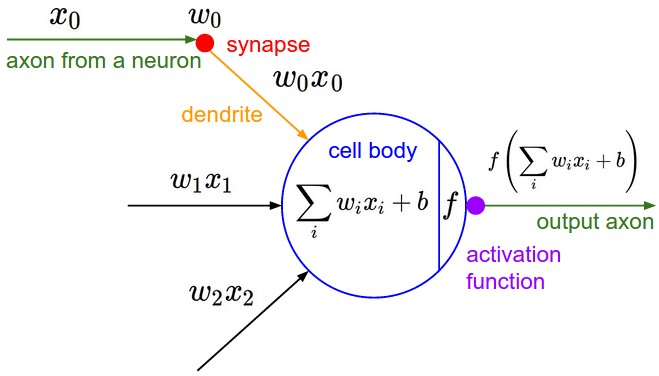
\includegraphics[scale=0.2, valign=t]{neuron_model}
\caption{Analogy between biological neuron and Rosenblatt's Perceptron (figures from \url{http://cs231n.github.io/neural-networks-1/})}
\label{perceptron}
\end{figure}

The analogy between biological neuron and Rosenblatt's Perceptron is depicted in Figure \ref{perceptron}.
Intuitively, Rosenblatt's Perceptron corresponds to a neuron, and an input $\bmx \subset \calx$ corresponds to impulses received by the neuron.
The weight $w_i$ corresponds to the connectivity strength of the $i$th synapsis, and the bias $b$ corresponds to stimulation strength that triggers the neuron.
In the case of perceptron, the activation function is $\sigma (x) = x$.
Other popular choices of activation function include
\begin{itemize}
\item the heaviside function $\sigma (x) = \ind_{x > 0}$
\item the sigmoid function $\sigma (x) = \frac1{1 + \exp (-x)}$
\item the hyperbolic tangent function $\sigma (x) = \tanh (x)$
\item the rectified linear unit (ReLU) $\sigma (x) = \max (0, x)$
\end{itemize}
The choice that these activation functions are bounded when $x \rightarrow \infty$, except for ReLU, resembles mechanisms in brain that maintain stability of the nervous system.

\subsubsection{The limitation of Rosenblatt's Perceptron: learning the \textsc{XOR} operation}

Consider the case $\calx = \{0, 1\}^2$, $\caly = \{0, 1\}$, $\bbp$ is uniform over $\calx$, and
\[
y(\bmx)
= y(x_1, x_2)
= \textsc{XOR} (x_1, x_2) \triangleq \ind_{x_1 = x_2}
\]
i.e. the XOR operation.
In this case, $\bmw = (w_1, w_2) \subset \bbr^2$ and
\[
h_{\bmw, b} (\bmx) = w_1 x_1 + w_2 x_2 + b
\]
Suppose we have obtained the ``perfect" sample, i.e. a sample that results in an empirical risk identical to the true risk
\[
\{((0, 0), 1), ((1, 0), 0), ((0, 1), 0), ((1, 1), 1)\} \subset \{0, 1\}^2 \times \{0, 1\}
\]
Clearly,
Thus Rosenblatt's Perceptron cannot learn the XOR operation, which is ubiquitous in many applications.

\subsection{Multi-layer Perceptron}

A solution to the aforementioned problem of Rosenblatt's Perceptron is to take a ``linear" combination of neurons with nonlinear activation function instead of only taking a ``linear" combination of input features, i.e. replacing Rosenblatt's Perceptron by two-layer neural network.
It could be helpful to think of these neurons as a basis.
Intuitively, this basis of neurons should be richer than the canonical basis of $\bbr^d$, and thus mappings not representable in the canonical basis of $\bbr^d$ may be representable in the basis of neurons.
Consequently, we may expect the hypothesis space of two-layer neural networks to be richer than the hypothesis space of perceptrons, and able to learn more complex mappings from the input space to the output space.
Mathematically, a two-layer neural network is
\[
g(\bmx) = \sum_{i = 1}^{d_1} v_i h_{\bmw_i, b_i} (\bmx) + a
\]
where
\[
h_{\bmw, b} (\bmx) = \sigma(\bmw^T \bmx + b)
\]
is a neuron, and $\bmw_i$ and $b_i$ are the weight and bias of the $i$th neuron.

A biological interpretation of two-layer neural network is a neuron that take as input the activation of other neurons.
Instead of being activated by input features, a neuron receives the activation of other neurons, which are activated by input features instead.

\begin{figure}
\centering
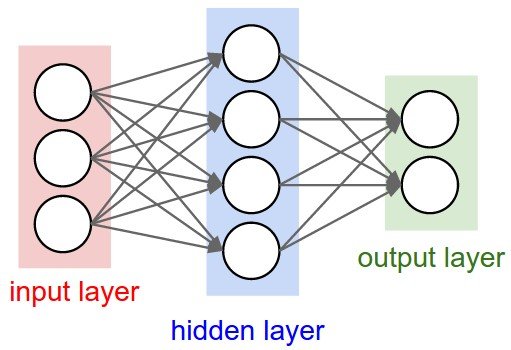
\includegraphics[scale=0.2, valign=t]{neural_net}
\caption{A neural network with one hidden layer (figure from \url{http://cs231n.github.io/neural-networks-1/})}
\end{figure}

\subsection{Vectorization}

We may write the computation of a neural network more compactly using matrix-vector multiplication, a.k.a. vectorization in the neural network community:
\[
g(\bmx)
= \sum_{i = 1}^{d_1} v_i h_{\bmw_i, b_i} (\bmx) + a
= \bmv^T \sigma (W \bmx + \bmb) + a
\]
where $\bmv = [v_1, ..., v_{d_1}]$, the $i$th row of $W \in \bbr^{d_1 \times d}$ is $\bmw_i$, and $\bmb = [b_1, ..., b_{d_1}]^T$.
For $\bmv \in \bbr^d$ and $\sigma: \bbr \mapsto \bbr$,
\[
\sigma (\bmv) \triangleq [\sigma (v_1), ..., \sigma (v_d)]^T
\]
$\sigma (W \bmx + \bmb)$ is the activation of the hidden layer because $\sigma (W \bmx + \bmb)_i$ is the activation of the $i$th neuron.

\subsection{Multi-dimensional output}

In order to construct a neural network that produces multi-dimensional output, one may replace $\bmv \in \bbr^{d_1}$ by $V \in \bbr^{d_1 \times d_2}$ and $a \in \bbr$ by $\bma \in \bbr^{d_2}$ if $\caly \subset \bbr^{d_2}$:
\[
g(\bmx) = V \sigma (W \bmx + \bmb) + \bma
\]
Intuitively, multiple perceptrons taking as input the activation of a collection of neurons (the $i$th row of $V$ and $a_i$ are the weight and bias of the $i$th perceptron).

\subsection{Multi-layer perceptron (MLP)}

Replace input layer by hidden layer, i.e. $\bmx$ by $\sigma (W \bmx + \bmb)$, again, again, and again \ldots
\begin{align*}
\bmh_0 & = \bmx \\
\bmh_i & = \sigma (W_i \bmh_{i - 1} + \bmb_i) \qquad i = 1, ..., L - 1 \\
g(\bmx) & = W_L \bmh_{L - 1} + \bmb_L
\end{align*}
where $h_i$ is the activation of the $i$th hidden layer.

\begin{figure}
\centering
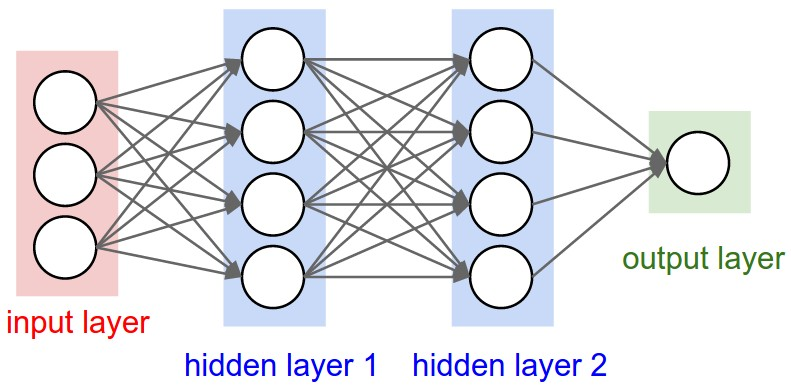
\includegraphics[scale=0.2, valign=t]{neural_net2}
\caption{An MLP with two hidden layers (figure from \url{http://cs231n.github.io/neural-networks-1/})}
\end{figure}

\subsection{Forward and backward propagation}

Given an input $x \in \bbr^d$, the forward propagation rule of a $L$-layer perceptron with weights $\{W^{(l)}\}_{l = 1}^L$, biases $\{b_l\}_{l = 1}^L$, and activation function $\sigma: \bbr \mapsto \bbr$ is defined as
\begin{alignat*}{2}
h_0 & \triangleq x \\
\bar{h}_l & \triangleq W^{(l)} h_{l - 1} + b_l && \qquad l \in [L - 1] \\
h_l & \triangleq \sigma (\bar{h}_l) && \qquad l \in [L - 1] \\
h_L & \triangleq W^{(L)} h_{L - 1} + b_L
\end{alignat*}
where $[n] \triangleq \{1, ..., n\}$, $W^{(l)} \in \bbr^{d_l \times d_{l - 1}}$ with $d_0 \triangleq d$, $b_l \in \bbr^{d_l}$, and the application of $\sigma$ is pointwise.

Given a supervision signal $y \in \caly$ and a loss function $\ell: \bbr^{d_L} \times \caly \mapsto \bbr$, backward propagation refers to the computation of $\{W^{(l)}'\}_{l = 1}^L$ and $\{b_l'\}$, where
\[
W_{i j}^{(l)}' \triangleq \pp{\ell}{W_{i j}^{(l)}} (h_L, y) \qquad
b_l' \triangleq \pp{\ell}{b_l} (h_L, y)
\]

Intuitively, the forward propagation computes the output of a neural network given its input, and the backward propagation computes gradient of a loss function with respect to the neural network's parameters.
It follows from the chain rule that the corresponding backward propagation rule is
\begin{alignat*}{2}
h_L' & \triangleq \nabla_{h_L} \ell (h_L, y) \\
W^{(L)}' & \triangleq \nabla_{W^{(L)}} \ell (h_L, y) = h_L' h_{L - 1}^T \\
b_L' & \triangleq \nabla_{b_L} \ell (h_L, y) = h_L' \\
h_{L - 1}' & \triangleq \nabla_{h_{L - 1}} \ell (h_L, y) = W^{(L) T} h_L' \\
\bar{h}_l' & \triangleq \nabla_{\bar{h}_l} \ell (h_L, y) = \diag (\sigma' (\bar{h}_l)) h_{l + 1}' && \qquad l \in [L - 1] \\
W^{(l)}' & \triangleq \nabla_{W^{(l)}} \ell (h_L, y) = \bar{h}_l' h_{l - 1}^T && \qquad l \in [L - 1] \\
b_l' & \triangleq \nabla_{b_l} \ell (h_L, y) = \bar{h}_l' && \qquad l \in [L - 1] \\
h_l' & \triangleq \nabla_{h_l} \ell (h_L, y) = W^{(l) T} \bar{h}_l' && \qquad l = 0, ..., L - 2
\end{alignat*}
where $\diag (x)_{i j} \triangleq x_i \delta_{i j}$ and the application of $\sigma'$ is again pointwise.

\subsection{The universal approximator theorem}

Define the hypothesis space of two-layer neural networks as
\[
\calh_{NN} \triangleq \{\text{neural network with one hidden layer}\}
\]
$\calh_{NN}$ is a hypothesis space much richer than the hypothesis space of perceptrons, mathematically characterized by the following theorems:
\begin{theorem}[Cybenko \cite{cybenko1989approximation}]
$\calh_{NN}$ is dense in $C ([0, 1]^d)$.
\end{theorem}

There is no free lunch!
PAC-learnability lost:
\begin{corollary}
\[
d_{VC} \left(\left\{\ind_{h(\cdot) > \frac12} : h \in \calh_{NN}\right\}\right) = \infty
\]
\end{corollary}
Essentially a consequence of the universal approximator theorem and the fact that $C ([0, 1]^d)$ shatters any finite subset of $[0, 1]^d$.

\begin{proof}
It suffices to prove that $\left\{\ind_{h(\cdot) > \frac12} : h \in \calh_{NN}\right\}$ shatters any finite subset of $[0, 1]^d$.
$\forall n \in \bbn$, $\forall E \triangleq \{x_i\}_{i = 1}^n \subset [0, 1]^d$, $\forall F \subset E$, $\exists f \in C([0, 1]^d)$ s.t.
\[
f(F) = \{1\} \qquad f(E - F) = \{0\}
\]
Because $\calh_{NN}$ is dense in $C([0, 1]^d)$, $\forall \epsilon > 0$, $\exists h \in \calh_{NN}$ s.t.
\[
\sup_{\bmx \in [0, 1]^d} |f(\bmx) - h(\bmx)| < \epsilon
\]
In particular, $\exists h \in \calh_{NN}$ s.t.
\[
\max_{\bmx \in E} |f(\bmx) - h(\bmx)| < \frac14
\]
\end{proof}

\subsection{VC-dimension and PAC-learnability}

The notion of VC-dimension was proposed by Vapnik and Chervonenkis in 1968 \cite{vapnik2015uniform}, which is the core of statistical learning theory.
\begin{definition}
The \emph{VC-dimension} of a hypothesis space $\calh$ is defined as
\[
d_{VC} (\calh) \triangleq \max \{n : \Pi_\calh (n) = 2^n\}
\]
where for $n \in \bbn$, the growth function of a hypothesis space $\calh$ is defined as
\[
\Pi_\calh (n) \triangleq \max_{\{x_i\}_{i = 1}^n \subset \calx} |\{h(x_i)\}_{i = 1}^n : h \in \calh\}|
\]
\end{definition}

In another language, $\calh$ shatters a set $\{x_i\}_{i = 1}^n$ if $|\{h(x_i)\}_{i = 1}^n : h \in \calh\}| = 2^n$, i.e. hypotheses in $\calh$ realize all possible binary labeling of the set $\{x_i\}_{i = 1}^n$.
By the definition of growth function, $\Pi_\calh (n) = 2^n$ if and only if $\calh$ shutters some subset of size $n$.
Thus the VC-dimension of $\calh$ is the greatest $n$ such that $\calh$ shatters some subset of size $n$.

\begin{theorem}
\[
d_{VC} (\calh) < \infty
\Leftrightarrow \calh\ \text{is PAC-learnable (by ERM)}
\]
\end{theorem}

\subsection{Solution to lost PAC-learnability: structural risk minimization (SRM) \cite{vapnik1992principles}}

The algorithm of structural risk minimization (SRM) is motivated by the following large deviation bound derived by Vapnik and Chervonenkis, which is the core of the VC-theory:
\begin{theorem}
Suppose $d_{VC} (\calh) < \infty$.
Then with probability at least $1 - \eta$,
\[
\forall h \in \calh, R (h) < \hat{R} (h) + \delta_\calh
\]
where
\[
\delta_\calh \triangleq \sqrt{\frac{d_{VC} (\calh) \left(\log \frac{2 n}{d_{VC} (\calh)} + 1\right) - \log \eta}{n}}
\]
\end{theorem}
The idea of SRM is that instead of minimizing the empirical risk, one may minimize the upper bound of the confidence interval.
Indeed, for a hypothesis space with finite VC-dimension, minimizing the empirical risk is equivalent ot minimizing the upper bound, because in this case the upper bound is merely the empirical risk plus a constant that only depends on the VC-dimension of the hypothesis space, the deviation and the level of confidence.
However, the idea of SRM becomes more interesting when the hypothesis space of interest has infinite VC-dimension because these hypothesis spaces typically are union of hypothesis spaces with finite VC-dimension.
In this case, one may apply the idea of SRM to select hypothesis from an increasing family of hypothesis spaces to guarantee some level of confidence in the generalization error.

Mathematically, suppose $\exists \calh_1 \subset \calh_2 \subset ...$ such that
\[
\calh = \bigcup_i^\infty \calh_i
\]
i.e. $\calh$ is a union of an increasing family of hypothesis spaces.
Define $h_i^*$ as the hypothesis in the hypothesis space $\calh_i$ with the minimum empirical risk, i.e.
\[
h_i^* \triangleq \argmin_{h \in \calh_i} \hat{R} (h)
\]
It follows the construction that
\[
\hat{R} (h_1^*) \leq \hat{R} (h_2^*) \leq \ldots \qquad
\]
Also,
\[
d_{VC} (\calh_1) \leq d_{VC} (\calh_2) \leq \ldots
\Rightarrow \delta_{\calh_1} \geq \delta_{\calh_2} \geq \ldots
\]

Because
\[
\forall h \in \calh, R (h) < \hat{R} (h) + \delta_\calh
\]
Hopefully the upper bound $\hat{R}(h_i^*) + \delta_{\calh_i}$ is a U-shaped function of $i$, which is analoguous to bias-variance trade-off.

Define
\[
U(i) \triangleq \hat{R}(h_i^*) + \delta_{h_i}
\]
It is clear that upper bound of the confidence interval as a U-shaped function can be optimized by the following algorithm:
\begin{algorithmic}
\STATE $i \gets 1$
\WHILE{$U(i) \leq U(i + 1)$}
    \STATE $i \gets i + 1$
\ENDWHILE
\RETURN $i$
\end{algorithmic}

Algorithmically, SRM is feasible as long as ERM is feasible, i.e. it is feasible to compute $h_i^*$.

\subsubsection{SRM applied to $\calh_{NN}$}

Let $\calh_{NN}^n \triangleq \{\text{neural network with one hidden layer of size}\ n\}$.
\[
\calh_{NN} = \bigcup_{n = 1}^\infty \calh_{NN}^n
\]

Consequence: neural networks with a fixed architecture is PAC-learable, and are not universal function approximators.
Gradient descent.

\subsubsection{SRM applied to $\calh_{NN}$ (continued)}

Apply SRM to the hypothesis familiy
\[
\calh_{NN}^1, \calh_{NN}^2, \ldots
\]
(although it is not the case that $\calh_{NN}^1 \subset \calh_{NN}^2 \subset \ldots$, why?)

It remains to compute
\[
h_i^* \triangleq \argmin_{h \in \calh_i} \hat{R} (h)
\]

\subsubsection{ERM with gradient descent}

As illustrated in class, fix $\calh_{NN}^i$ we can optimize
\[
\frac1n \sum_{i = 1}^n \ell(g(\bmx_i), y_i)
\]
with gradient descent for ``nice" surrogate loss functions $\ell$, although the optimization problem now is always non-convex.

However, you can still give it a try!

We can use the chain rule to compute gradient (a.k.a. backward propagation).
Hopefully you have mastered the chain rule by now. If not \ldots

\subsubsection{Limitation of SRM}

Cohen et al. shows that ``[B]esides a negligible set, all functions that can be implemented by a deep network of polynomial size, require exponential size in order to be realized (or even approximated) by a shallow network."\cite{cohen2016expressive}

Consider neurons $\{f_{\bmw, b}\}$ a basis indexed by $\bmw \in \bbr^d$ and $b \in \bbr$.
A complete basis can have high approximation complexity for some functions.

Forget about \emph{universal} approximators and instead look for ``good" (in the language of mathematicians) bases/(in the language of alchemists) architectures!

What does ``good" mean?

\subsection{The VC-dimension of multi-layer perceptrons}

Each $\calh_{NN}^n$ is a more restricted hypothesis space:
\begin{theorem}[Karpinski and Macintyr \cite{maass1995vapnik}]
If $\sigma (x) = 1 / (1 + \exp (-x))$, then
\[
d_{VC} (\calh_{NN}^n) = \calo (m^4)
\]
where $m$ is the number of weights.
\end{theorem}

\section{Neural networks for structured data}

Structured data refers to data representable as a mapping $\Omega \mapsto \bbr^d$.
For example, in the case of sequential/temporal data, $\Omega$ is real intervals representing time;
in the case of image data, $\Omega$ is rectangles in $\bbr^2$;
in the case of graph data, $\Omega$ is a graph.

\subsection{Recurrent neural networks: neural networks for sequential/temporal data}

An example of sequential data is sentences in natural languages.
A natural motivation for the architecture of recurrent neural network (RNN) is the following.
Suppose we are trying to evaluate the probability for a sequence $\{x_t\}_{t = 1}^T \subset \bbr^d$ to occur.
It follows from the definition of conditional probability that
The motivation for RNN is to summarize $\{X_s = x_s : s < t\}$, i.e. the conditions at time $t$, by a vector $h_t \in \bbr^H$, and approximate.
The simplest
\[
W_x x + W
\]
\[
\bbp (X_1 = x_1, ..., X_T = x_T)
= \prod_{t = 1}^T \bbp (X_t = x_t | X_s = x_s\ \text{for}\ s < t)
\]
It is crucial that the number of parameters in recurrent neural networks is independent from the sequence length $T$, which enables RNN's to handle long sequences.
The performance of RNN depends significantly on how well the vector $h_t$ summarizes the conditions at time $t$.
It turns out that the simplest RNN can easily "forget" conditions in distant past.
One possible remedy is the long short term memory (LSTM) network, defined as
\begin{align*}
f_t & = \sigma (W_f x_t + U_f h_{t - 1} + b_f) \\
i_t & = \sigma (W_i x_t + U_i h_{t - 1} + b_i) \\
o_t & = \sigma (W_o x_t + U_o h_{t - 1} + b_o) \\
c_t & = f_t \odot c_{t - 1} + i_t \odot \sigma_c (W_c x_t + U_c h_{t - 1} + b_c) \\
h_t & = o_t \odot \sigma_h (c_t)
\end{align*}
where $\odot$ denotes the Hadamard product, $\sigma$ denotes the sigmoid function, $\sigma_c = \tanh$, and $\sigma_h$ is either $\tanh$ or the identity function.
$f$, $i$, and $o$ respectively refer to the forget gate, input gate, and output gate.
The heuristic of LSTM is to control how the internal state $c$ is forgot, enriched, and output by gating.
A simplification of LSTM is the gated recurrent unit (GRU), defined as
\begin{align*}
z_t & = \sigma (W_z x_t + U_z h_{t - 1} + b_z) \\
r_t & = \sigma (W_r x_t + U_r h_{t - 1} + b_r) \\
h_t & = (1 - z_t) \odot h_{t - 1} + z_t \sigma_h (W_h x_t + U_h (r_t \odot h_{t - 1}) + b_h)
\end{align*}
where $z$ and $r$ refer to the update and reset gate.

\subsection{Basics of harmonic analysis}

\begin{definition}
The Fourier transform $\calf f$ of $f \in L^1 (\bbr^d)$ is defined as
\[
(\calf f) (\bmxi) \triangleq \int_{\bbr^d} e^{-i \bmxi^T \bmx} f(\bmx) \dif \bmx
\]
The inverse Fourier transform $\calf f$ of $f \in L^1 (\bbr^d)$ is defined as
\[
(\calf f) (\bmx) \triangleq \int_{\bbr^d} e^{i \bmx^T \bmxi} f(\bmxi) \dif \bmxi
\]
\end{definition}

It follows from the definition that $\calf f \in L^\infty (\bbr^d)$ for $f \in L^1 (\bbr^d)$ because
\begin{align*}
|f|_{L^\infty (\bbr^d)}
& = \sup_{\xi \in \bbr^d} |(\calf f) (\xi)| \\
& = \sup_{\xi \in \bbr^d} \left|\int_{\bbr^d} e^{-i \xi x} f(x) \dif x \right| \\
& \leq \sup_{\xi \in \bbr^d} \int_{\bbr^d} \left|e^{-i \xi x} f(x) \right| \dif x \\
& = \sup_{\xi \in \bbr^d} \int_{\bbr^d} |f(x)| \dif x \\
& = |f|_{L^1 (\bbr^d)}
\end{align*}
where $\sup$ denotes the essential supremum, as in the definition of $L^\infty (\bbr^d)$.

$L^2 (\bbr^d)$ is a Hilbert space when equipped with the inner product
\[
\langle f, g\rangle_{L^2 (\bbr^d)} \triangleq \int_{\bbr^d} f \bar{g} \dif \mu \qquad f, g \in L^2 (\bbr^d)
\]
where $\mu$ denotes the Lebesgue measure of $\bbr^d$, which follows from the fact that the norm induced by $\langle \cdot, \cdot\ranglq_{L^2 (\bbr^d)}$ coincides with $|\cdot|_{L^2 (\bbr^d)}^2$, and $L^2$ equipped with $|\cdot|_{L^2 (\bbr^d)}^2$ is a Banach space.

In the following, we multiply the Lebesgue measure by the constant $\frac1{\sqrt{(2 \pi)^d}}$.
The Plancherel theorem asserts that the Fourier transform is an isometry.
\begin{theorem}[Plancherel]
\[
\langle f, g\rangle_{L^2 (\bbr^d)} = \langle \calf f, \calf g\rangle_{L^2 (\bbr^d)} \qquad \forall f, g \in L^1 (\bbr^d) \cap L^2 (\bbr^d)
\]
\end{theorem}

\begin{lemma}
$L^1 (\bbr^d) \cap L^2 (\bbr^d)$ is dense in $L^2 (\bbr^d)$.
\end{lemma}

\begin{proof}
For $f \in L^2 (\bbr^d)$, let
\[
f_n (x) = f(x) \ind_{|x| < n}
\]
By construction,
\[
\lim_{n \rightarrow \infty} f_n (x) = f(x) \qquad x \in \bbr^d
\]
By the triangle inequality,
\[
|f - f_n|
\leq |f| + |f_n|
\leq 2 |f|
\]
Furthermore, $\{f_n\}_{n = 1}^\infty \subset L^2 (\bbr^d)$ because it follows from the fact $f \in L^1 (\bbr^d)$ that $f$ has to be bounded on any subset of $\bbr^d$ with finite measure, and in particular the subsets $\{x : |x| < n\}$.
By the dominated convergence theorem,
\[
\lim_{n \rightarrow \infty} \int_{\bbr^d} |f - f_n|^2 \dif x
= \int_{\bbr^d} \lim_{n \rightarrow \infty} |f - f_n|^2 \dif x
= 0
\]
where the dominating function is $4|f|^2$, which implies that
\[
\lim_{n \rightarrow \infty} |f - f_n| = 0
\]
Because the choice of $f$ is arbitrary, we conclude that $L^1 (\bbr^d) \cap L^2 (\bbr^d)$ is dense in $L^2 (\bbr^d)$.
\end{proof}

\begin{lemma}
For $1 \leq p < \infty$ and $f \in L^p (\bbr)$, $\calt_x: \bbr \mapsto L^p (\bbr)$ is uniformly continuous.
\end{lemma}

% We are now ready to prove the Plancherel theorem.
% 
% \begin{proof}
% For $f \in L^1 (\bbr^d) \cap L^2 (\bbr^d)$, let
% \[
% g(x) = <\calt_{-x} f, f>_{L^2 (\bbr^d)}
% \]
% \end{proof}

Consequently, $\calf f$ for $f \in L^2 (\bbr^d) - L^1 (\bbr^d)$ can be defined as the limit of
\[
\{\calf f_n\}_{n = 1}^\infty \subset L^1 (\bbr^d) \cap L^2 (\bbr^d)
\]
where $f_n \rightarrow f$ and convergence is in the $L^2$-norm.
Because $L^1 (\bbr^d) \cap L^2 (\bbr^d)$ is dense in $L^2 (\bbr^d)$, a sequence $\{f_n\}_{n = 1}^\infty$ that converges to $f$ in the $L^2$-norm indeed exsists.
Because a convergent sequence has to be a Cauchy sequence,
\[
\forall \epsilon > 0, \exists N \in \bbn, m, n > N \Rightarrow |f_m - f_n|_{L^2 (\bbr^d)} < \epsilon
\]
Because the Fourier transform is an isometry for $f \in L^1 (\bbr^d) \cap L^2 (\bbr^d)$,
\[
\forall \epsilon > 0, \exists N \in \bbn, m, n > N \Rightarrow |\calf (f_m - f_n)|_{L^2 (\bbr^d)} = |\calf f_m - \calf f_n|_{L^2 (\bbr^d)} < \epsilon
\]
Consequently, $\{\calf f_n\}_{n = 1}^\infty$ is a Cauchy sequence, and it follows from the Plancherel theorem that
\[
\{\calf f_n\}_{n = 1}^\infty \subset L^1 (\bbr^d) \cap L^2 (\bbr^d)
\]
Because $L^2 (\bbr^d)$ is a Hilbert space, in which every Cauchy sequence converges, the limit of $\{\calf f_n\}_{n = 1}^\infty$ is well-defined.

A fundamental property of the Fourier transform is that smoothness in the spatial domain implies decay in the frequency domain.
To state it in a general setting, we introduce the following definitions.
Given a $d$-dimensional multi-index $\alpha = (\alpha_1, ..., \alpha_d) \in \bbn^d$, the differential operator $D^\alpha$ is defined as
\[
D^\alpha \triangleq \frac{\partial^{\alpha_1}}{\partial x_1^{\alpha_1}} \cdot \ldots \cdot \frac{\partial^{\alpha_d}}{\partial x_d^{\alpha_d}}
\]
The order $|\alpha|$ of $\alpha$ is defined as
\[
|\alpha| \triangleq \sum_{i = 1}^d \alpha^i
\]
Define
\[
\calc^k \triangleq \{f : D^\alpha f\ \text{is continuous for all}\ |\alpha| \leq k\}
\]
We restrict $D^\alpha$ to $\calc^{|\alpha|}$, so that the ordering of partial differential operators in the definition of $D^{\alpha}$ does not matter by Schwarz's theorem.
For $1 \leq p \leq \infty$ and $k \in \bbn$, the ($L^p$)-Sobolev space of order $k$ is defined as
\[
W_p^k \triangleq \{f \in L^p : D^\alpha f \in L^p\ \text{for all}\ |\alpha| \leq k\}
\]
Stoke's theorem states that
\[
\int_\Omega \dif \omega = \int_{\partial \Omega} \omega
\]

The Laplacian is defined as
\[
\Delta \triangleq \sum_{i = 1}^d \frac{\partial^2}{\partial x_i^2}
\]
For a function $u: \bbr^{d + 1} \mapsto \bbr$, where the first $d$ dimensions are spatial and the last dimension is temporal, the heat equation is
\[
\pp{u}{t} = c \Delta u
\]

\subsection{Convolution}

\begin{definition}
The convolution $k * f$ of $f \in L^1 (\bbr^d) \cap L^2 (\bbr^d)$ with $k \in L^1 (\bbr^d) \cap L^2 (\bbr^d)$ is defined as
\[
(k * f) (\bmy) \triangleq \int_{\bbr^d} k(\bmy - \bmx) f(\bmx) \dif \bmx
\]
where $f$ is interpreted as a signal (e.g. an image), and $k$ is interpreted as a kernel.
\end{definition}

The convolution theorem asserts that convolution in the spatial domain coincides with multiplication in the frequency domain.
\begin{theorem}
\[
k * f = \calf^{-1} ((\calf k) \cdot (\calf f))
\]
\end{theorem}

For signal localized in the frequency domain, we may choose the kernel $k$ to be a smooth function such that its Fourier transform is localized in the frequency domain.
Then convolving a signal $f$ with the kernel $k$ effectively truncates the frequency spectrum of $f$.
However, the technique of truncation is ineffective for image.
Indeed, perhaps the most elementary component of an image is its edges, mathematically representable as indicator functions $\ind_{[-T, T]}$.
It is well-known that
\[
\calf \ind_{[-T, T]} (\xi)
= \int_{-\infty}^\infty e^{-i \xi x} \ind_{[-T, T]} (x) \dif x
= \int_{-T}^T e^{-i \xi x} \dif x
= \frac{2 \sin (T \xi)}\xi
\]
which implies that truncating the frequency spectrum of $\ind_{[-T, T]}$ causes significant loss of information.
Consequently, in order to retrieve information encoded in the tail of signal's tail frequency spectrum, one has to choose a kernel $k$ such that its fourier transform $\calf k$ does not vanish at the tail of signal's frequency spectrum.
In the case of convolutional neural networks, the kernels (a.k.a. filters) are chosen to have very compact support, which ensures that they have non-vanishing Fourier transforms by the Heisenberg uncertainty principle.

In the following we summarize an argument that motivates the transition from Fourier to Littlewood-Paley wavelets in computer vision.
The Fourier transform modulus is translation invariant.
Indeed,
\[
|\calf \calt_x f| (\xi)
= |e^{-i x^T \xi} (\calf f) (\xi)|
= |(\calf f) (\xi)|
\]
However, at high frequencies, deformations may cause instabilities.
Consider the scaling deformation field defined as
\[
\tau (x) = s x
\]
for a constant $|s| < 1$.
Note that
\[
|\nabla \tau| = |s| < 1
\]
\[
L_\tau f(x) = f(x - \tau (x)) = f((1 - s) x)
\]
Consider the signal $f(x) = e^{i \xi^T x} \theta (x)$, where $\theta$ is a regular function with fast decay.
It is clear that there is instability when $\xi \rightarrow \infty$.

\subsection{Convolutional neural networks (CNN) for image classification}

An image is a mapping $f: \bbr^2 \rightarrow \bbr^C$ with compact support, where $C$ is the number of channels ($C = 1$ for grayscale image, $C = 3$ for RBG image).

Assume the support is $[0, 1]^2$.

After discretizing $[0, 1]^2$: $\bmx \in \bbr^{W H C}$.

\subsubsection{Discretized convolution}

A fundamental building block of CNN's is the convolution layer, which is the discretization of the aforementioned convolution operator.
As described previously, in order to capture edges, which have non-vanishing Fourier transform, one has to choose a compactly-supported kernel.
Indeed, a convolution layers is typically equipped with a kernel of size $3 \times 3$ or $5 \times 5$, where the numbers refer to the number of pixels.
In some cases, one may choose a convolution kernel of size $1 \times 1$, which is equivalent to an affine transformation along the feature dimension.
Apart from the size of convolution kernel, other hyperparameters involved are stride and padding.
Stride refers to the rate at which the kernel scans the image.
Padding deals with the boundary cases, i.e. whether pixels at the boundary of the image are to be discarded.

A convolution layer is illustrated in Figure \ref{conv}.
Because the kernel essentially implements an affine transformation, it can be interpreted as a neuron as well.
However, this neuron is only ``locally connected", in the sense that it only receives impulses from pixels within its sliding window.
Like neurons in multi-layer perceptron, this convolution neuron can also be equipped with a non-linear activation function, and its activation can be received by other neurons as well.

\begin{figure}
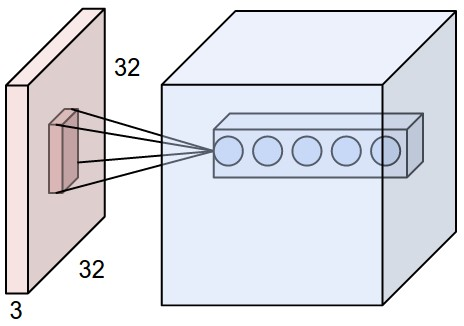
\includegraphics[scale=0.2]{depthcol}
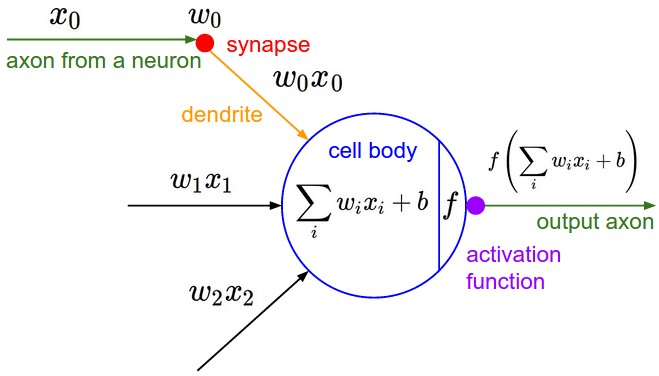
\includegraphics[scale=0.2]{neuron_model}
\caption{Convolution (figure from \url{http://cs231n.github.io/convolutional-networks/})}
\label{conv}
\end{figure}

\subsubsection{Downsampling tricks}

In many cases it would be helpful to downsample an image, i.e. to create an representation of an image with smaller size.
The trick in the literature of neural networks for this is pooling.
To downsample an image, one partition the image into grids, and apply a reducer to pixels in each grid.
Common reducers are mean and maximum, resulting respectively in the average and maximum pooling.
The only hyperparameter one has to control is the ``kernel size", which in fact refers to the size of grid.
The most common choices of grid size are $2 \times 2$ and $3 \times 3$ (pixels).
Note that the pooling layer is completely non-parametric.

Pooling is illustrated with an image of size $4 \times 4$ and $2 \times 2$ maximum pooling in Figure \ref{pool}.

Pooling is the key to translation invariance for CNN's.
Through pooling, the correspondence between information and its spatial location is progressively lost, resulting in translation-invariant high-level representations that can be handled by a MLP or even perceptron.

\begin{figure}
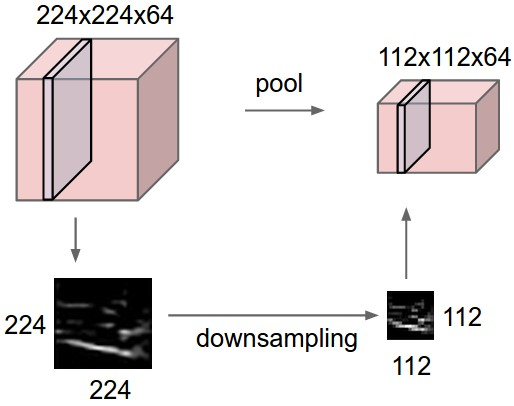
\includegraphics[scale=0.2]{pool}
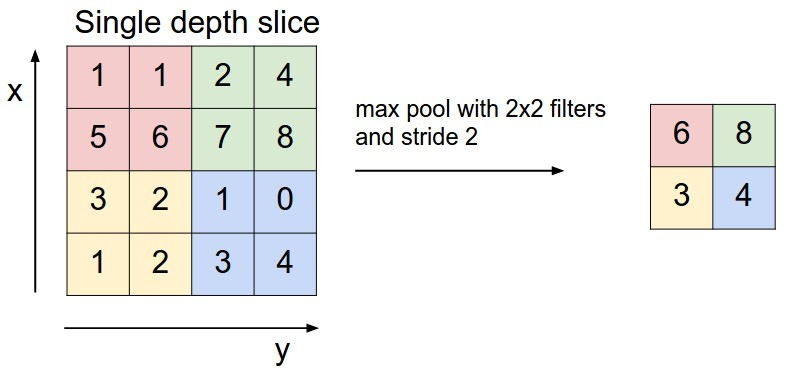
\includegraphics[scale=0.2]{maxpool}
\caption{Pooling (figure from \url{http://cs231n.github.io/convolutional-networks/})}
\label{pool}
\end{figure}

\subsubsection{Example: LeNet}

LeNet was proposed by LeCun et al. for the task of grey-scale digit recognition \cite{lecun1998gradient}.
Its architecture is illustrated in Figure \ref{lenet}.
It consists of two convolution layers, each followed by a downsampling layer.
The convolution and downsampling layers are followed by fully connected layers.

\begin{figure}
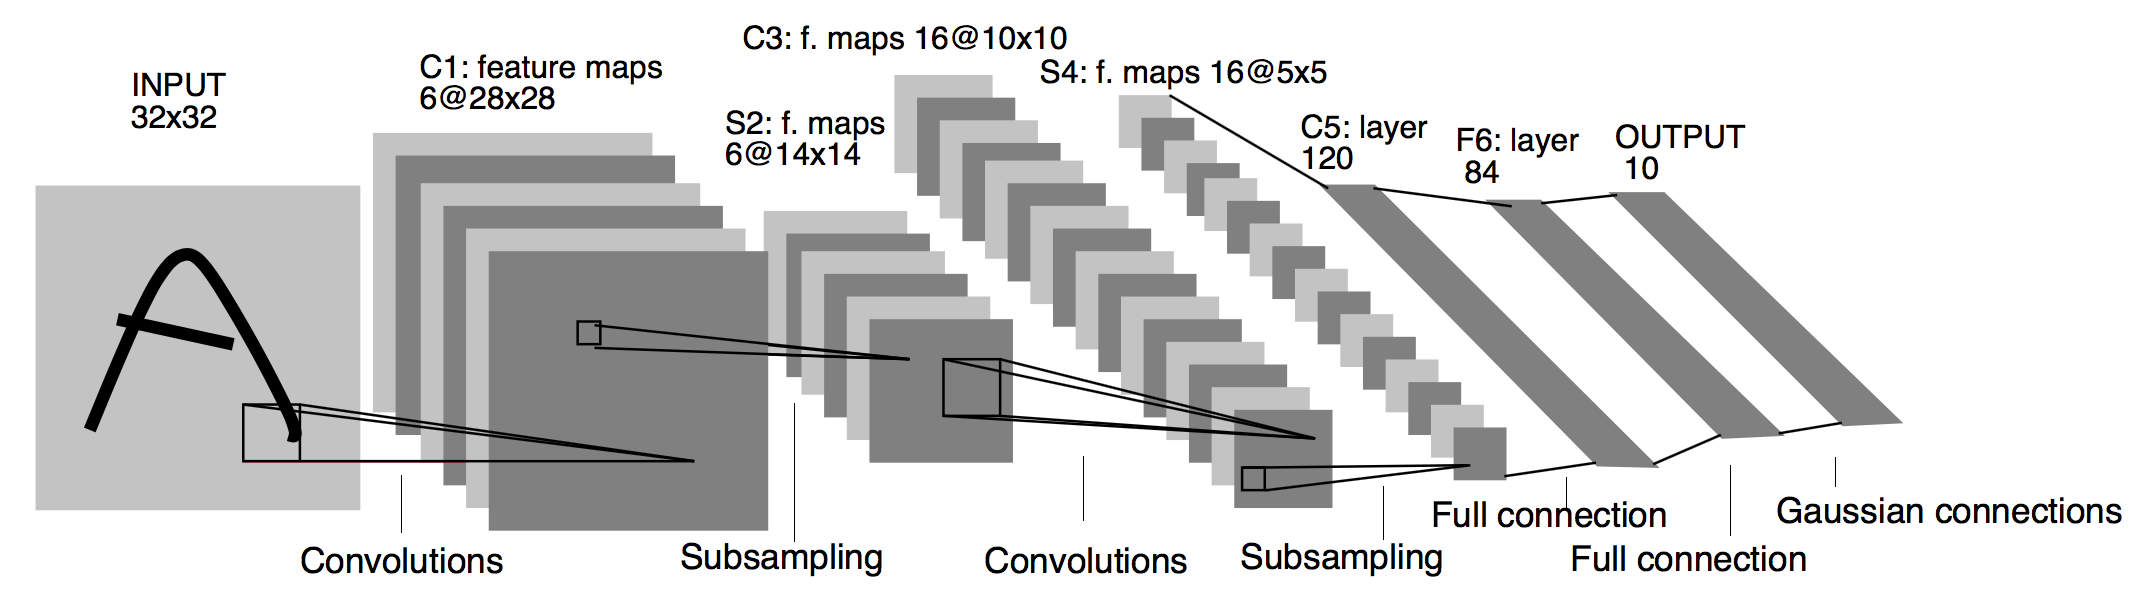
\includegraphics[scale=0.1]{lenet}
\caption{The architecture of LeNet (figure from \cite{lecun1998gradient})}
\label{lenet}
\end{figure}

\subsection{Deformation invariance}

Ideally, any image processor should be invariant under the translation and local deformation of images, which are ubiquitous in nature.
More precisely, we would like our image processor to produce identical results for translated images, while the results for generally deformed images should be proportional to the extent of deformation.
In the following we describe a mathematical formulation of this idea.

The mathematical abstraction of translation/deformation is a displacement/deformation field:
\[
\tau: \bbr^d \mapsto \bbr^d \in \calc^2
\]
where $\calc^2$ refers to vector fields with continuous second partial derivatives.
The displacement/deformation operator corresponding to a displacement/deformation field is defined as
\[
(\call_\tau f) (\bmx) \triangleq f(\bmx - \tau (\bmx))
\]
which deforms an image with a displacement/deformation field.
In the simple case of translation, the displacement field is simply a constant
\[
\tau (\bmx) = \bmc \qquad
(\call_\tau f) (\bmx) = f(\bmx - \bmc)
\]

Mathematically, an image processor can be considered as an operator in $L^2 (\bbr^2)$.
An operator $\Phi$ is translation invariant if
\[
\Phi \call_\tau f = \Phi f
\]
for all images $f \in L^2 (\bbr^d)$.
An operator $\Phi$ is translation equi-variant if
\[
\Phi \call_\tau f = \call_\tau \Phi f
\]
for all images $f \in L^2 (\bbr^d)$.

Convolution is translation equi-variant because
\begin{align*}
(k * (\call_\tau f)) (\bmy)
& = \int_{\bbr^d} k(\bmx) (\call_\tau f) (\bmy - \bmx) \dif \bmx \\
& = \int_{\bbr^d} k(\bmx) f(\bmy - \bmx - \bmc) \dif \bmx \\
& = \int_{\bbr^d} k(\bmx) f((\bmy - \bmc) - \bmx) \dif \bmx \\
& = (k * f) (\bmy - \bmc) \\
& = (\call_\tau (k * f)) (\bmy)
\end{align*}

Clearly, MLP is neither translation invariant nor translation equi-variant.

It remains an open question for what kind of kernels is convolution deformation-invariant.

Mallat shows how to construct a deformation-invariant kernel \cite{mallat2012group}.

However, is it the best kernel?

Learning with information bottleneck may result in better kernels.

\subsubsection{Non-parametric convolutional neural networks}

It turns out that for some simple tasks, e.g. MNIST digit recognition, convolutional neural networks without learnable parameters can achieve state of the art performance as well.
In the following we describe the architecture of PCANet \cite{chan2015pcanet}, a convolutional neural network with filters inferred solely from Principle Component Analysis (PCA).
Consider a dataset consisting of $n$ image-label pairs
\[
\{(x_i, y_i)\}_{i \in [n]} \subset \bbr^{W H C} \times \caly
\]
where $W$, $H$, and $C$ are the width, height, and number of channels of images, and $\caly$ is the collection of labels.
Suppose the filter (patch) $W$ has size $k_w \times k_h$.
The parameters of the filter is computed by applying PCA to the vectors
\[
\bigcup_{i = 1}^n \{x_{i, j}\}_{j = 1}^{k_w k_h}
\]
where $x_{i, pq}$ denotes the $k_w \times k_h$ patch with top left corner located at pixel $(p, q)$ of image $x_i$.
Suppose the number of output channels is $C'$.
Then retain the leading $C'$ eigenvectors of the corresponding covariance matrix as filter.
Such "PCAConv" layers can be cascaded.

\subsection{Deep learning on graphs}

In the following we describe neural networks tailored to data with graph structures.
More precisely, we are interested in data representable as $\calv \mapsto \bbr^d$ for some graph $\calg = (\calv, \cale)$.
We shall assume that both $\calv$ and $\cale$ are finite and adopt the convention that $n \triangleq |\calv|$ and $m \triangleq |\cale|$.
We shall identify $\calv$ with $[n]$ and $\cale$ with $[m]$.
We assume that $\calg$ is undirected, i.e. $(i, j) \in \cale \Leftrightarrow (j, i) \in \cale$ for all $i, j \in \calv$.
We assume that $\calg$ has no self-connection, i.e. $(i, i) \ne \cale$ for $i \in [n]$.
Let $M_i$ denote the $i$-th row of $M$, and $M^i$ denote the $i$-th column of $M$.

\subsubsection{Laplacian on graphs}

A real-valued function (signal) on $\calg = (\calv, \cale)$ is a mapping $\calv \mapsto \bbr$, which can be identified with a vector in $\bbr^n$ by identifying $\calv$ with $[n]$.
We assume that along with $\calg$ comes a real symmetric matrix $W$ and $W_{i j}$ is a positive number interpreted as the strength of connection between $i, j \in \calv$.
The degree of $i \in \calv$ is defined as
\[
\degree (i) \triangleq \sum_{j = 1}^n W_{i j}
\]
and the degree matrix $D$ of $\calg$ is an $n \times n$ diagonal matrix defined as
\[
D_{i j} \triangleq \delta_{i j} \degree (i)
\]
The Laplacian of $\calg$ is defined as
\[
L \triangleq D - W
\]
An alternative motivation for the definition of graph Laplacian is the following.
Suppose $u: \calv \times \bbr \mapsto \bbr$ describes the evolution of heat distribution over $\calv$.
Newton's law of cooling states that the heat transferred between $i, j \in \calv$ in an infinitestimal period of time is proportional to the difference $u_i - u_j$ when $(i, j) \in \cale$.
Consequently,
\begin{align*}
\pp{u_i}{t}
& = -c \sum_{(i, j) \in \cale} w_{i j} (u_i - u_j) \\
& = -c \left(\degree (i) u_i - \sum_{(i, j) \in \cale} w_{i j} u_j\right)
\end{align*}
Vectorizing the identity, we have
\begin{align*}
\pp{u}{t}
& = -c (D u - A u) \\
& = -c (D - A) u \\
& = -c L u
\end{align*}

\subsubsection{Convolution on graphs}

\begin{equation*}
f * g (x) \triangleq \int_{\bbr^d} f(y) (\calt_x (\calr g)) (y) dy
\end{equation*}
where $(\calr g) (\cdot) \triangleq g(-\cdot)$ is the reflection operator and $(\calt_x g) (\cdot) \triangleq g(x + \cdot)$ is the translation (by $x$) operator.
Neither $\calr$ nor $\calt_x$ makes sense when we replace $\bbr^d$ by $\calg$.
\begin{equation*}
f * g = \calf^{-1} (\calf  f \calf g)
\end{equation*}

Other definitions of Laplacian exists in the literature.
For example, the random walk Laplacian is defined as
\[
L^{RW} \triangleq I - W D^{-1}
\]
However, the random walk Laplacian is in general asymmetric and thus unsuitable for our purpose.
It follows from the spectral theorem for real symmetric matrix that $L$ admits the decomposition
\begin{equation*}
L = U^T \Lambda U
\end{equation*}
where $U \in SO(n)$, $L U_i = \Lambda_{i i} U_i$ for $i \in [n]$, $\Lambda$ is diagonal, and $\Lambda_{i i} \leq \Lambda_{j j} \forall 1 \leq i < j \leq n$.
\begin{equation*}
(U f)_i
= f^T U_i
= <f, U_i>_{\bbr^b}
\end{equation*}
which is analoguous to
\begin{equation*}
(\calf f) (n)
\triangleq \int_T e^{-i n x)} f(x) \dif x
= <e^{-i n \cdot}, f>_{L^2}
\end{equation*}
We can define Fourier transform $\calf$ on $\calg$ analoguously as
\begin{equation*}
\calf f \triangleq U f
\end{equation*}
Because $U^T U = I$ on $\bbr^n$ and $\calf^{-1} \calf = I$ on $L^2$, a natural definition for inverse Fourier transform on $\calg$ is
\begin{equation*}
\calf^{-1} \triangleq U^T
\end{equation*}

\begin{equation*}
f * g
\triangleq \calf^{-1} (\calf f \cdot \calf g)
= U^T (U f \odot U g)
\end{equation*}
where $\odot$ denotes the Hadamard product.
Analoguous to the approach to convolution on image, one of $f$ and $g$ filter and the other signal.
In the following let $x$ denote a signal and $\theta$ denote a filter.
\[
\theta * x
= U^T (U \theta \odot U x)
\]
Because $U \in SO(n)$,
\[
\theta * x
= U^T (\theta \odot U x)
= U^T (\diag (\theta) U x)
\]
(possibly with nonlinearity attached)

However, this construction has two disadvantages.
First,
Second, computing the eigen-decomposition $U^T \Lambda U$ is expensive.
One solution, proposed by \cite{defferrard2016convolutional}, is to replace $\diag (\theta)$ with a polynomial of $\Lambda$ with learnable coefficient.
Suppose $\Theta = \sum_{k = 0}^K \theta_k \Lambda^k$.
\begin{align*}
\Theta * x
& = U^T \Theta U x \\
& = U^T \left(\sum_{k = 0}^K \theta_k \Lambda^k \right) U x \\
& = \left(\sum_{k = 0}^K \theta_k U^T \Lambda^k U \right) x \\
& = \sum_{k = 0}^K \theta_k L^k x
\end{align*}
where the last identity follows from the fact that
\[
L L
= U^T \Lambda U U^T \Lambda U
= U^T \Lambda^2 U
\]
It follows from the definition of $L$ that $L$ contains $n + 2 m$ non-zero entries, which is significantly less than $n^2$ when $\calg$ is sparse, i.e. when $m / n^2 \rightarrow 0$.
An efficient implementation of $L x$, commonly referred to as Sparse Matrix-Vector multiplication (SpMV), only requires $\calo ()$ time.
Truncating higher order terms in the expansion results in the popular Graph Convolutional Network (GCN) \cite{kipf2016semi}.

In the following we describe a neural network architecture motivated by an improved spectral clustering algorithm.

A natural setting for theoretical analysis of spectral clustering algorithms is the Stochastic Block Model (SBM).
In the binary case, given a collection of nodes $\calv = [n]$ and a label assignment $\sigma: \calv \mapsto {\pm 1}$, the probability for two nodes $i, j \in \calv$ to be connected is
\[
\bbp [(i, j) \in \cale]
= \ind_{\sigma_i = \sigma_j} p_{in} + \ind_{\sigma_i \ne \sigma_j} p_{out}
\]
where $p_{in}$ denotes the probability of an inter-community edge and $p_{out}$ denotes the probability of an extra-community edge.
To model sparse graphs, let
\[
p_{in} = \frac{c_{in}}n \qquad
p_{out} = \frac{c_{out}}n
\]
where $c_{in}$ and $c_{out}$ are constants, and $n \rightarrow \infty$.
detectability threshold:
\[
c_{in} - c_{out}
\]
SBM can model many real world graphs, in particular, social networks.
"Birds of a feather flock together."
Importantly, many real world graphs have bounded maximum degree when $n \rightarrow \infty$, i.e.
\[
d^* \triangleq \lim_{n \rightarrow \infty} \max_{i \in \calv} \degree (i) < \infty
\]
These graphs are sparse because
\[
\frac{m}{n^2}
\leq \frac{d^* n}{n^2}
= \frac{d^*}n
\]

It turns out that standard spectral clustering fails at the limit $n \rightarrow \infty$ even if detectable.

\section{Optimization of neural networks}

\subsection{Stochastic gradient descent}

\begin{theorem}[Convergenc of SGD for strongly convex problems with fixed step sizes]
Suppose $F$ is $\mu$-strongly convex.
If $\eta_t = \eta \leq \frac1{L c_g}$, then
\[
\bbe (F(x^t) - F(x^*)) \leq \frac{\eta L \sigma_g^2}{2 \mu} + (1 - \eta \mu)^t (F(x^0) - F(x^*))
\]
\end{theorem}

\begin{theorem}[Convergenc of SGD for strongly convex problems with diminishing step sizes]
Suppose $F$ is $\mu$-strongly convex, and $c_g = 0$.
If $\eta_t = \frac\theta{t + 1}$ for some $\theta > \frac1{2 \mu}$, then
\[
\bbe |x^t - x^*|^2 \leq \frac{c_\theta}{t + 1}
\]
\end{theorem}

\begin{theorem}[Convergenc of SGD for convex problems]
Suppose $F$ is convex.
Let
\[
\bar{x}^t = \sum_{k = 0}^t \frac{\eta_k}{\sum_{j = 0}^t \eta_j} x^k
\]
Then
\[
\bbe (F(\bar{x}^t) - F(x^*)) \leq \frac{\bbe |x^0 - x^*|^2 + \frac12 \sigma_g^2 \sum_{k = 0}^t \eta_k^2}{2 \sum_{k = 0}^t \eta_k}
\]
\end{theorem}

\subsection{A toy example}

In the following we present the analysis of LeCun et al. \cite{le1991eigenvalues}.
Consider the dataset
\[
\{(x_i, y_i)\}_{i = 1}^n \subset \bbr^d \times \bbr
\]
a linear "neural network"
\[
f(x) = w^T x \qquad w \in \bbr^{d}
\]
and the mean square error as objective
\[
\ell (w) = \sum_{i = 1}^n (f(x_i) - y_i)^2
\]
It follows from linear algebra manipulations that
\begin{align*}
\ell (w)
& = \frac1n \sum_{i = 1}^n (f(x_i) - y_i)^2 \\
& = \frac1n \sum_{i = 1}^n (w^T x_i - y_i)^2 \\
& = \frac1n \sum_{i = 1}^n (w^T x_i - y_i) (x_i^T w - y_i) \\
& = \frac1n \sum_{i = 1}^n w^T x_i x_i^T w - 2 y_i w^T x_i + y_i^2 \\
& = w^T \left(\frac1n \sum_{i = 1}^n x_i x_i^T\right) w - \frac{2 w^T}n \sum_{i = 1}^n y_i x_i + \frac1n \sum_{i = 1}^n y_i^2 \\
& = w^T R w - 2 w^T q + c
\end{align*}
where
\[
R \triangleq \frac1n \sum_{i = 1}^n x_i x_i^T
\]
is the sample covariance matrix and
\[
q \triangleq \frac1n \sum_{i = 1}^n y_i x_i
\]
Because
\[
\nabla_w \ell (w) = 2 R w - 2 q
\]
the critical points are solution to the linear system
\[
R w = q
\]
Because $R$ is a square matrix, $R$ is injective if and only if $R$ is surjective.
It follows that when $R$ is injective, $q \in \range R$ and the solution is unique.
Otherwise, it may be the case that either $q \not \in \range R$, or
% argmin?
The corresponding Hessian is
\[
H (w) = 2 R
\]
The sample covariance matrix $R$ is real symmetric and thus has the eigen-decomposition
\[
R = U^T \Lambda U
\]
where $\Lambda$ is diagonal and the rows of $U$ is an orthonormal basis of $\bbr^d$.
In the basis, the convergence of SGD depends only on the ratio
\[
\frac{\lambda_{min}}{\lambda_{max}}
\]
which suggests that normalizing the input helps convergence.

\bibliographystyle{unsrt}
\bibliography{written}

\end{document}
